\documentclass{article}
\usepackage{ctex}

\usepackage{tikz}
\usetikzlibrary{graphs}

\begin{document}
    % 向量
    \begin{tikzpicture}
    \draw [color=blue!50, ->]
        (0,0)
        node [left] {$A$} -- 
        node [color=red!70, pos=0.5, above,sloped] {Hello} (3,3) 
        node [right] {$B$};
    \end{tikzpicture}

    % 圆,椭圆,矩形,贝塞尔曲线,扇形
    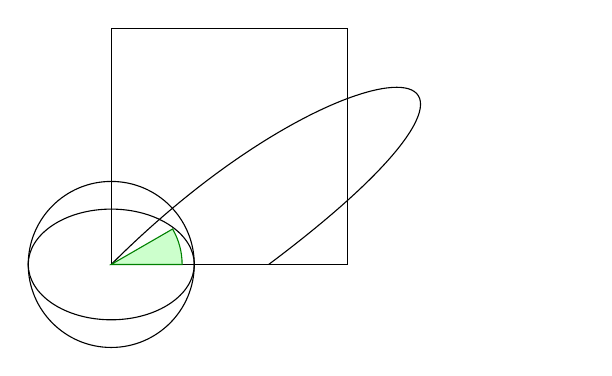
\begin{tikzpicture}
        \draw (0, 0) circle (30pt);
        \draw (0, 0) ellipse (30pt and 20pt);
        \draw (0, 0) rectangle (3, 3);
        \draw (0, 0) ..controls (3, 3) and (6, 3) .. (2, 0);
        \filldraw [fill=green!20!white, draw=green!50!black]
            (0, 0) -- (9mm, 0mm) arc (0:30:9mm) -- cycle; % 起始角度,终了角度,半径?
    \end{tikzpicture}

    \begin{tikzpicture}
        [
            L1Node/.style = 
                {circle, draw=blue!50,fill=blue!20
                very thick, minimum size=10mm},
            L2Node/.style = 
                {rectangle, draw=green!50, fill=green!20,
                very thick, minimum size=10mm}
        ]
    \end{tikzpicture}
\end{document}